\section{AIS Tradeflows}

AIS Trade Flow systems utilize data transmitted by vessels worldwide to offer real-time and historical insights into maritime trade activities.
The objective is to establish a system that defines trade between ports based on AIS signals.
Defining port areas within AIS Trade Flow systems is a complex process that takes into account both geographical and operational considerations.
Geographically, a port area is typically defined by a specific set of coordinates that delineate the physical boundaries of the port and its surrounding waters.
This definition may encompass berths, anchorages, and sometimes even approach channels. Determining whether a ship is within a port area often involves comparing the ship's current AIS-reported coordinates with the defined boundaries of the port.
If the ship's position falls within these boundaries, it is considered to be inside the port area. However, the determination is not solely based on geographical location.
Operational factors also come into play.
For instance, a ship may be within the geographical boundaries of a port, but if it is merely passing through without stopping or engaging in port activities, it may not be considered "in port" from an operational perspective.

To address these complexities, AIS Trade Flow systems frequently employ sophisticated algorithms to accurately establish port boundaries and classify vessel behavior.
These algorithms take into account various factors such as the ship's speed, course, and historical behavior patterns.
By integrating these diverse data points, these systems can provide a highly accurate depiction of port activities and vessel movements.
Astrup Feanley Code has developed a system based on these general principles, resulting in a dataset that encompasses AIS signals as well as information on port stops, loading, and unloading.


Vessels typically travel from one port to another, and these types of journeys are called port-to-port voyages.
Port-to-port voyages are categorized into two types: laden and ballast.
A laden voyage refers to a maritime journey undertaken by a vessel when it is carrying cargo.
This means that the ship is not empty but is loaded with goods or freight that is being trans- ported from one location to another.
On the other hand, a ballast voyage refers to a maritime journey in which a vessel travels without any cargo.
In this case, the ship is not carrying freight and is being transported from one location to another.

Thus, trade flow is comprised of one or more port-to-port voyages, which can either be laden or ballast.

(Explain figure showing tradeflow)

To achive this, the AIS data is processed to identify port-to-port voyages and then stored them in a database based on segments as shown in the Figure \ref{ais_processing}.

\begin{figure}[h]
    \centering
    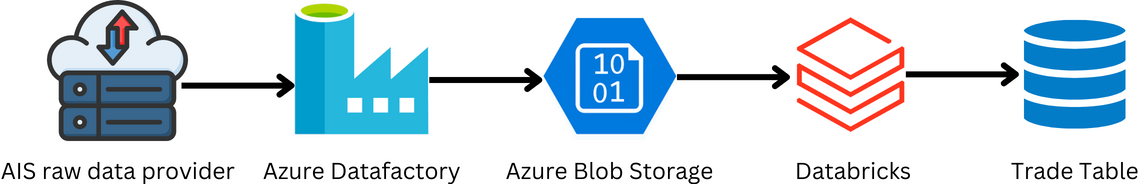
\includegraphics{images/ais_processing.png}
    \caption{AIS Raw Data Processing}
    \label{ais_processing}
\end{figure}

\subsection{Processing Raw AIS data to Trade Flow}

Astrup fearnley receives raw AIS data from external vendor called Exact Earth.
For this there is a pipeline setup on Azure Data Factory which updates raw data every hour in CSV files.

Using databricks following informations are extracted from the raw data and processed further:

\begin{table}[ht]
    \centering
    \small % reduce font size
    \begin{tabular}{|l|p{0.4\linewidth}|l|}
        \hline
        Column              & Description                                                      & Data Type               \\
        \hline
        IMO                 & International Maritime Organization 2                            & Number                  \\
        \hline
        \text{TS\_POS\_UTC} & Date and Time of Last Position AIS Message in UTC                & YYYYMMDDHHmmSS          \\
        \hline
        POSITION            & WGS84 Point, Geographic Location                                 & Geometry                \\
        \hline
        LONGITUDE           & WGS 84 Longitude Coordinate 2                                    & Number, Decimal Degrees \\
        \hline
        LATITUDE            & WGS 84 Latitude Coordinate                                       & Number, Decimal Degrees \\
        \hline
        SOG                 & Speed over Ground                                                & Number, Knots           \\
        \hline
        HEADING             & Heading                                                          & Number, Degrees         \\
        \hline
        \text{NAV\_STATUS}  & Navigational Status                                              & Text                    \\
        \hline
        DESTINATION         & Port of Destination                                              & Text                    \\
        \hline
        ETA                 & Month, Day, Hour, and Minute of Estimated Time of Arrival in UTC & MMDDHHmm                \\
        \hline
        DRAUGHT             & Vessel Draught                                                   & Number, Metres          \\
        \hline
    \end{tabular}
    \caption{Important data from raw AIS data}
    \label{tab:ais_raw_data}
\end{table}
